\subsection{The charged Higgs boson}
\label{sec:cHtheory}
\par Unlike the Standard Model Higgs boson mass, the charged Higgs boson mass is a free parameter 
in the 2HDM. As already mentioned, $\tan\beta$ is also a free parameter. Analyses presented in this 
text scan through the mass of the charged Higgs boson. Expanding Equation~\ref{eq:yk} reveals that 
couplings to fermions, $g_{\Hplus}(ud)$, are dependent on $\tan\beta$:

\begin{equation}
g_{\Hplus}(ud) = m_d\tan\beta(1+\gamma_5) + m_u\cot\beta(1-\gamma_5)
\end{equation} 

Figure~\ref{fig:chargedHverts} shows the allowed vertices between \Hplus\ and fermions, as 
well as with the SM Higgs boson $h$.  

\begin{figure}[!h]
\begin{subfigure}{0.33\textwidth}
   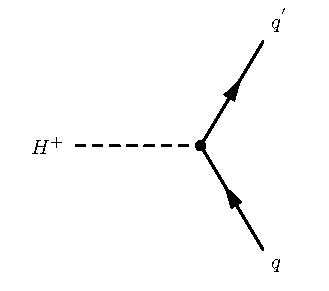
\includegraphics[width=\textwidth]{figures/chargedHq2.pdf}
\end{subfigure} % 
\begin{subfigure}{0.33\textwidth}
   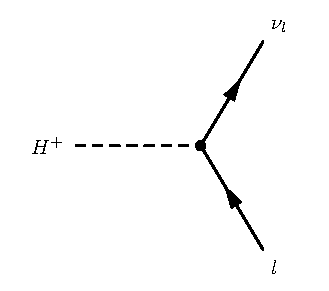
\includegraphics[width=\textwidth]{figures/chargedHlep.pdf}
\end{subfigure}%
\begin{subfigure}{0.33\textwidth}
   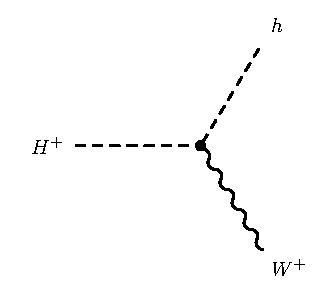
\includegraphics[width=\textwidth]{figures/chargedHh.pdf}
\end{subfigure}%
\caption{Feynman diagrams showing tree level charged Higgs vertices}
\label{fig:chargedHverts}
\end{figure}

\subsubsection{Production \& decay in $pp$ collisions}
\par Production of the charged Higgs boson from $pp$ collisions depends on its mass, $m_{H^{+}}$.
For $m_{H^{+}}$ less than the mass of the $t$ quark, $m_t$, the dominant mode of production is 
through the \tHb\ process.  For $m_{H^{+}}$ greater than $m_t$ production of the charged Higgs 
in association with a top quark is dominant. Figure~\ref{fig:chargedFeyn} shows such tree-level 
diagrams. The most dominant process for $t$ production is $gg\rightarrow\ttbar$ (known as \ttbar);

\begin{figure}[!h]
\centering
\begin{subfigure}{0.3\textwidth}
   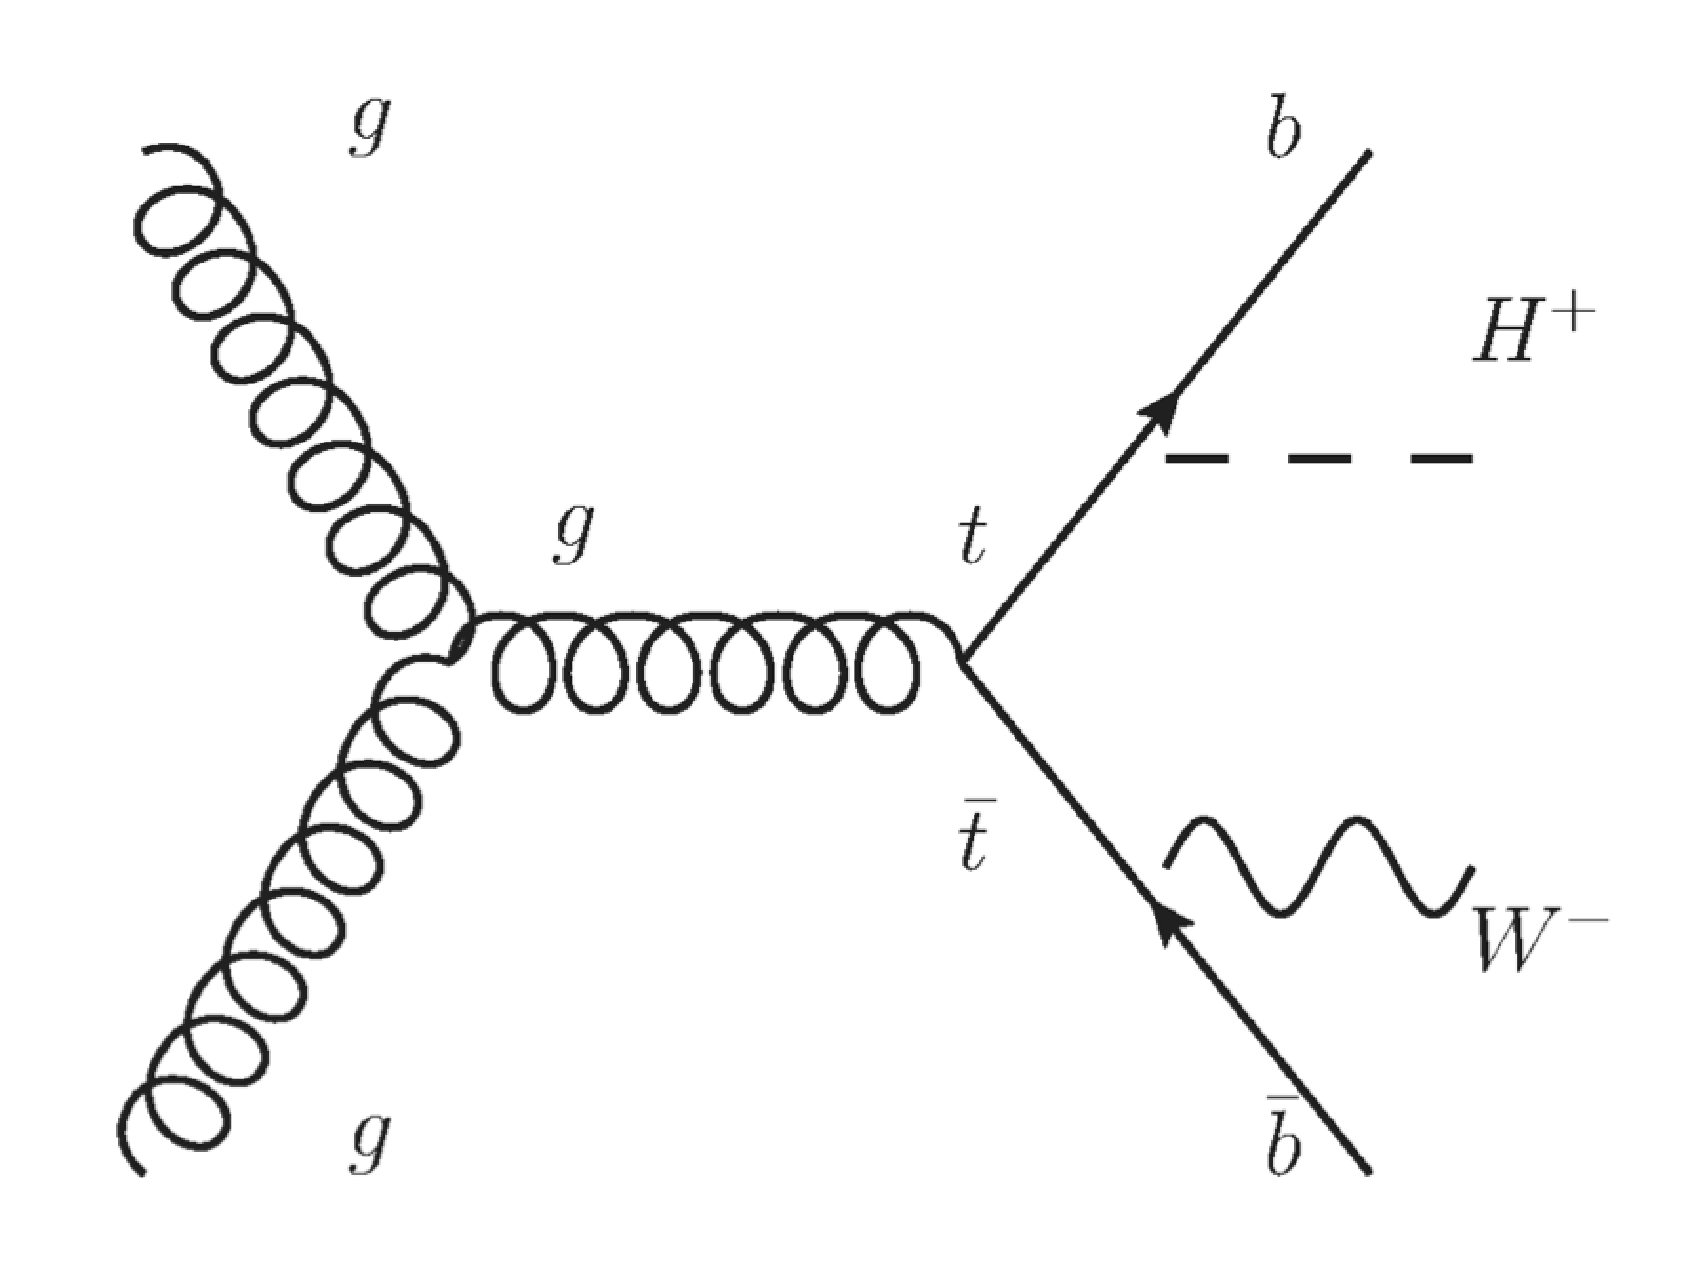
\includegraphics[width=\textwidth]{figures/feynmanIa.eps}
\caption{Top decay} 
\end{subfigure} % 
\begin{subfigure}{0.3\textwidth}
   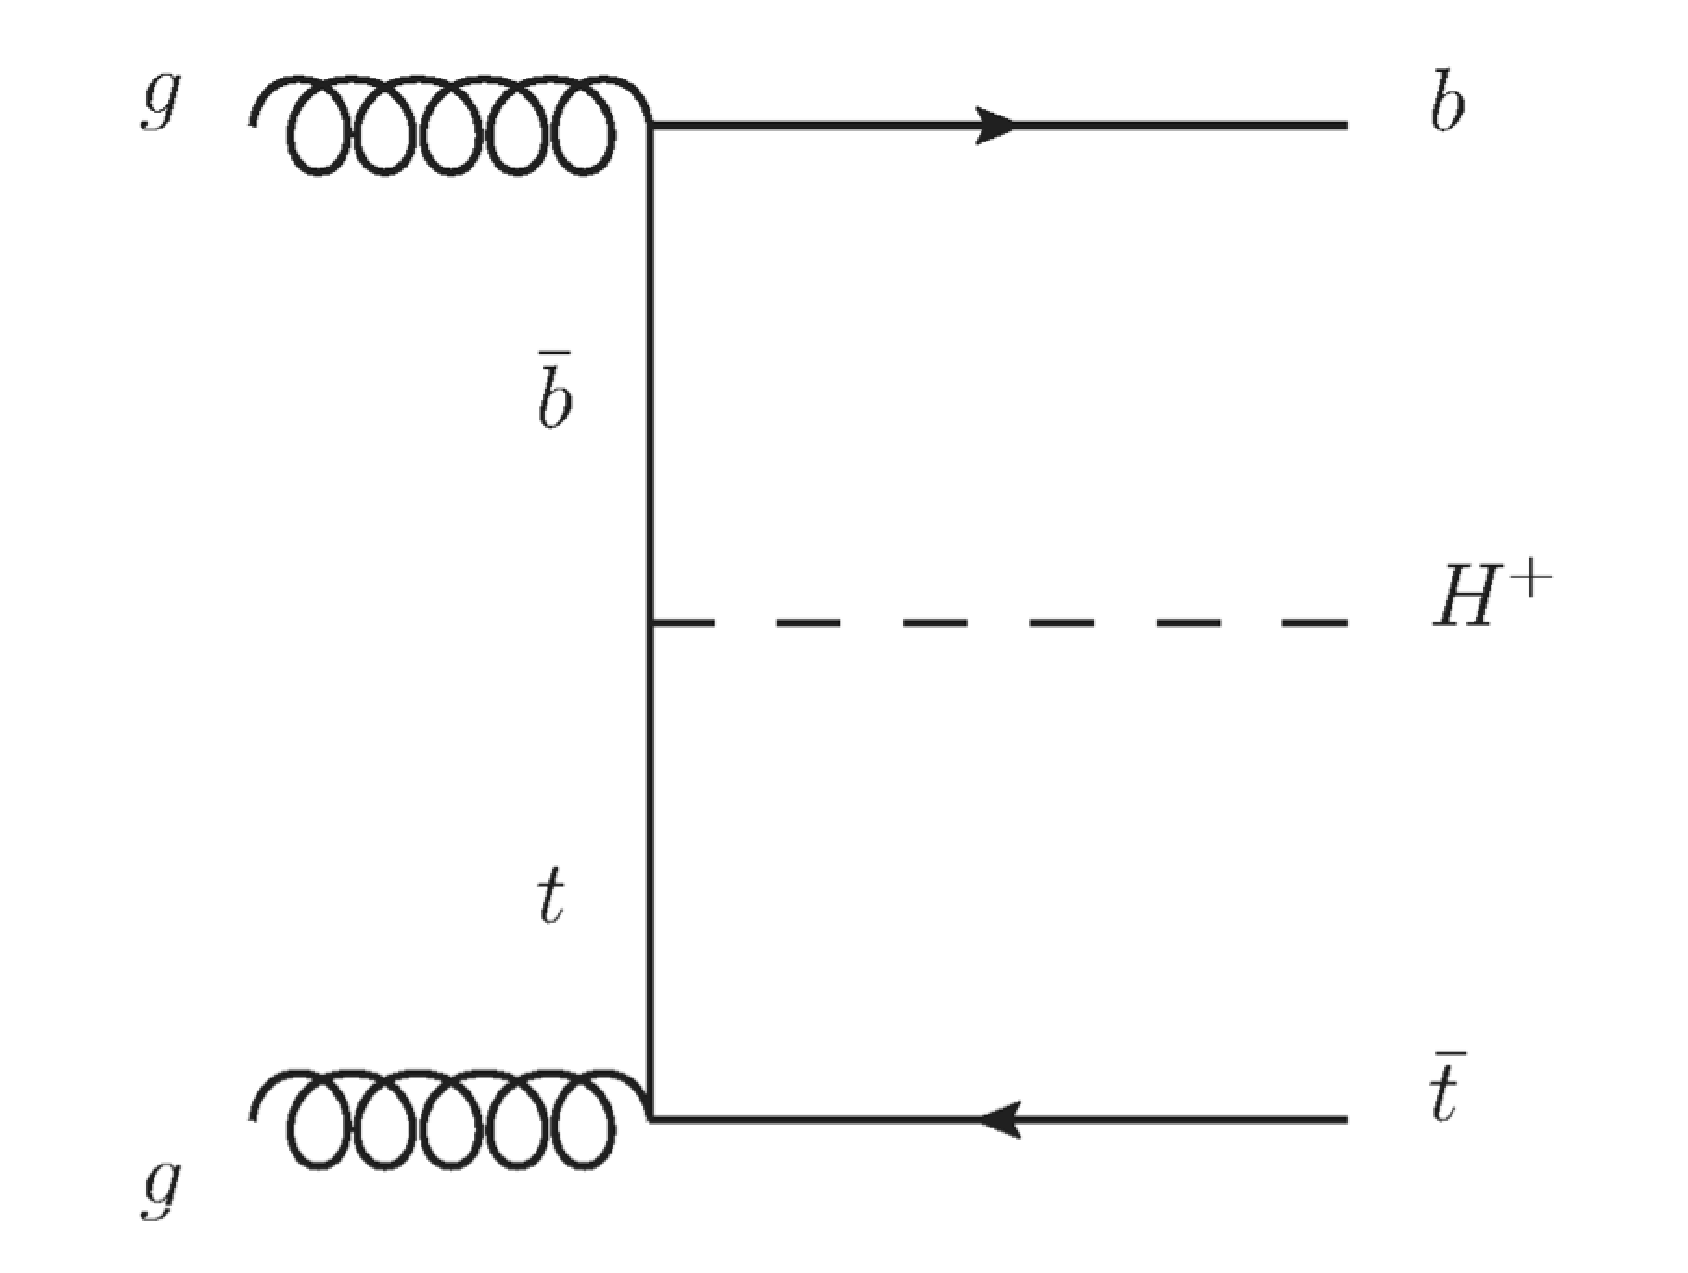
\includegraphics[width=\textwidth]{figures/feynmanIIIa.eps}
\caption{Top association -- 4FS}
\end{subfigure} % 
\begin{subfigure}{0.3\textwidth}
   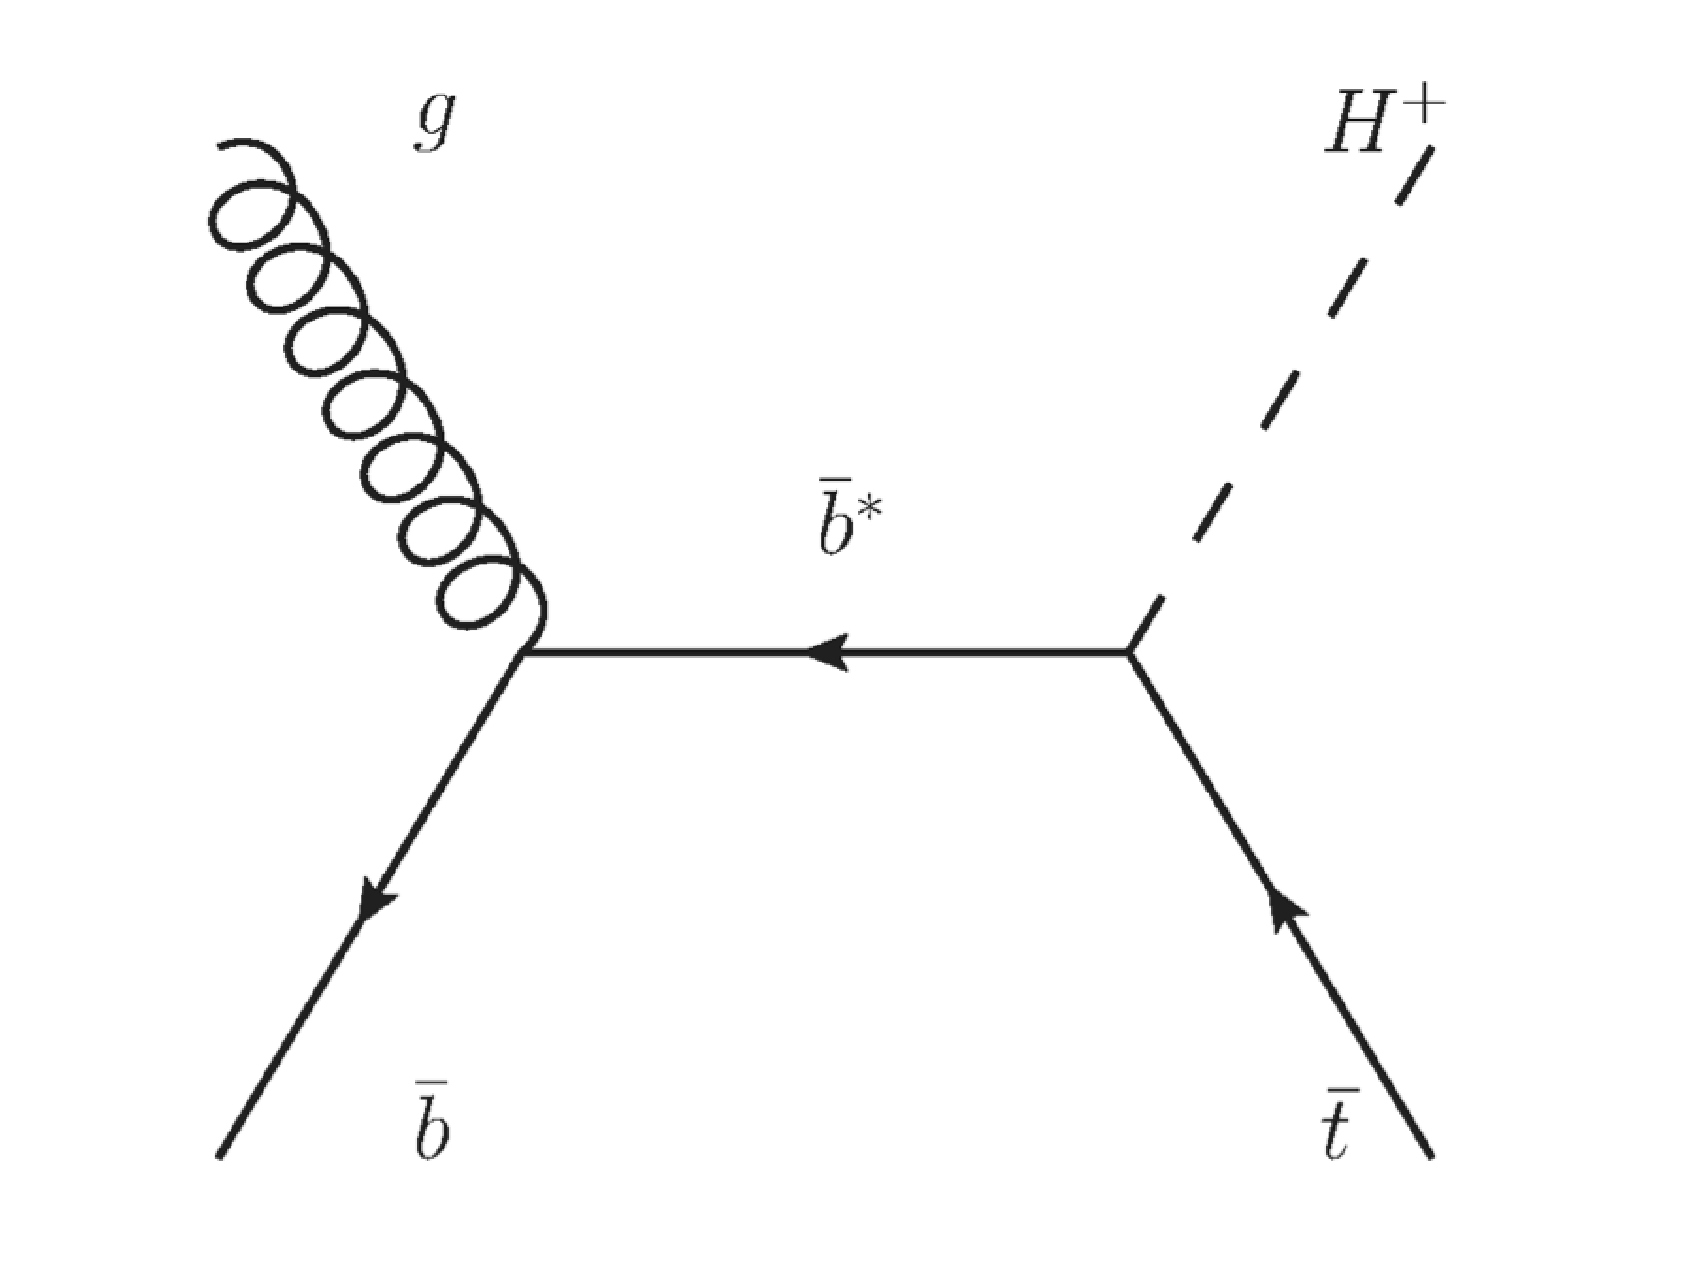
\includegraphics[width=\textwidth]{figures/feynmanIIa.eps}
\caption{Top association -- 5FS}
\end{subfigure} %
\caption{Feynman diagrams showing charged Higgs production}
\label{fig:chargedFeyn}
\end{figure}

\par For $m_{H^{+}}<m_t$ the charged Higgs is produced when one of the $t$ decays to a bottom quark. 
Clearly \ttbar\ events constitute a major background to the charged Higgs when conducting a search. 
When calculating amplitudes for these production vertices, the quark family is assummed to contain just 4
flavors of quarks $(u,d,c,s)$. The $b$ quark is included in the models only when it is necessary. 
For $m_{H^{+}}>m_t$ production can be through $gb\rightarrow tH^+$. Since the $b$ is included in this 
process, the scheme is known as the 5=flavor scheme. A 4-flavor scheme is $gg\rightarrow tbH^+$. 
Using $m_t$ as a boundary, charged Higgs bosons with mass less than 165~\GeV are referred to as {\it light}; 
those with mass greater than 200~\GeV are {\it heavy}, otherwise they are {\it intermediate}.

\par Figure~\ref{fig:chargedHxs} shows the total production cross section for a charged Higgs with 
$\mcH=200~\GeV$ plotted against $\tan\beta$, produced at $pp$ collision center-of-mass energy of $\sqs=13~\TeV$. 

\begin{figure}[h]
\centering
   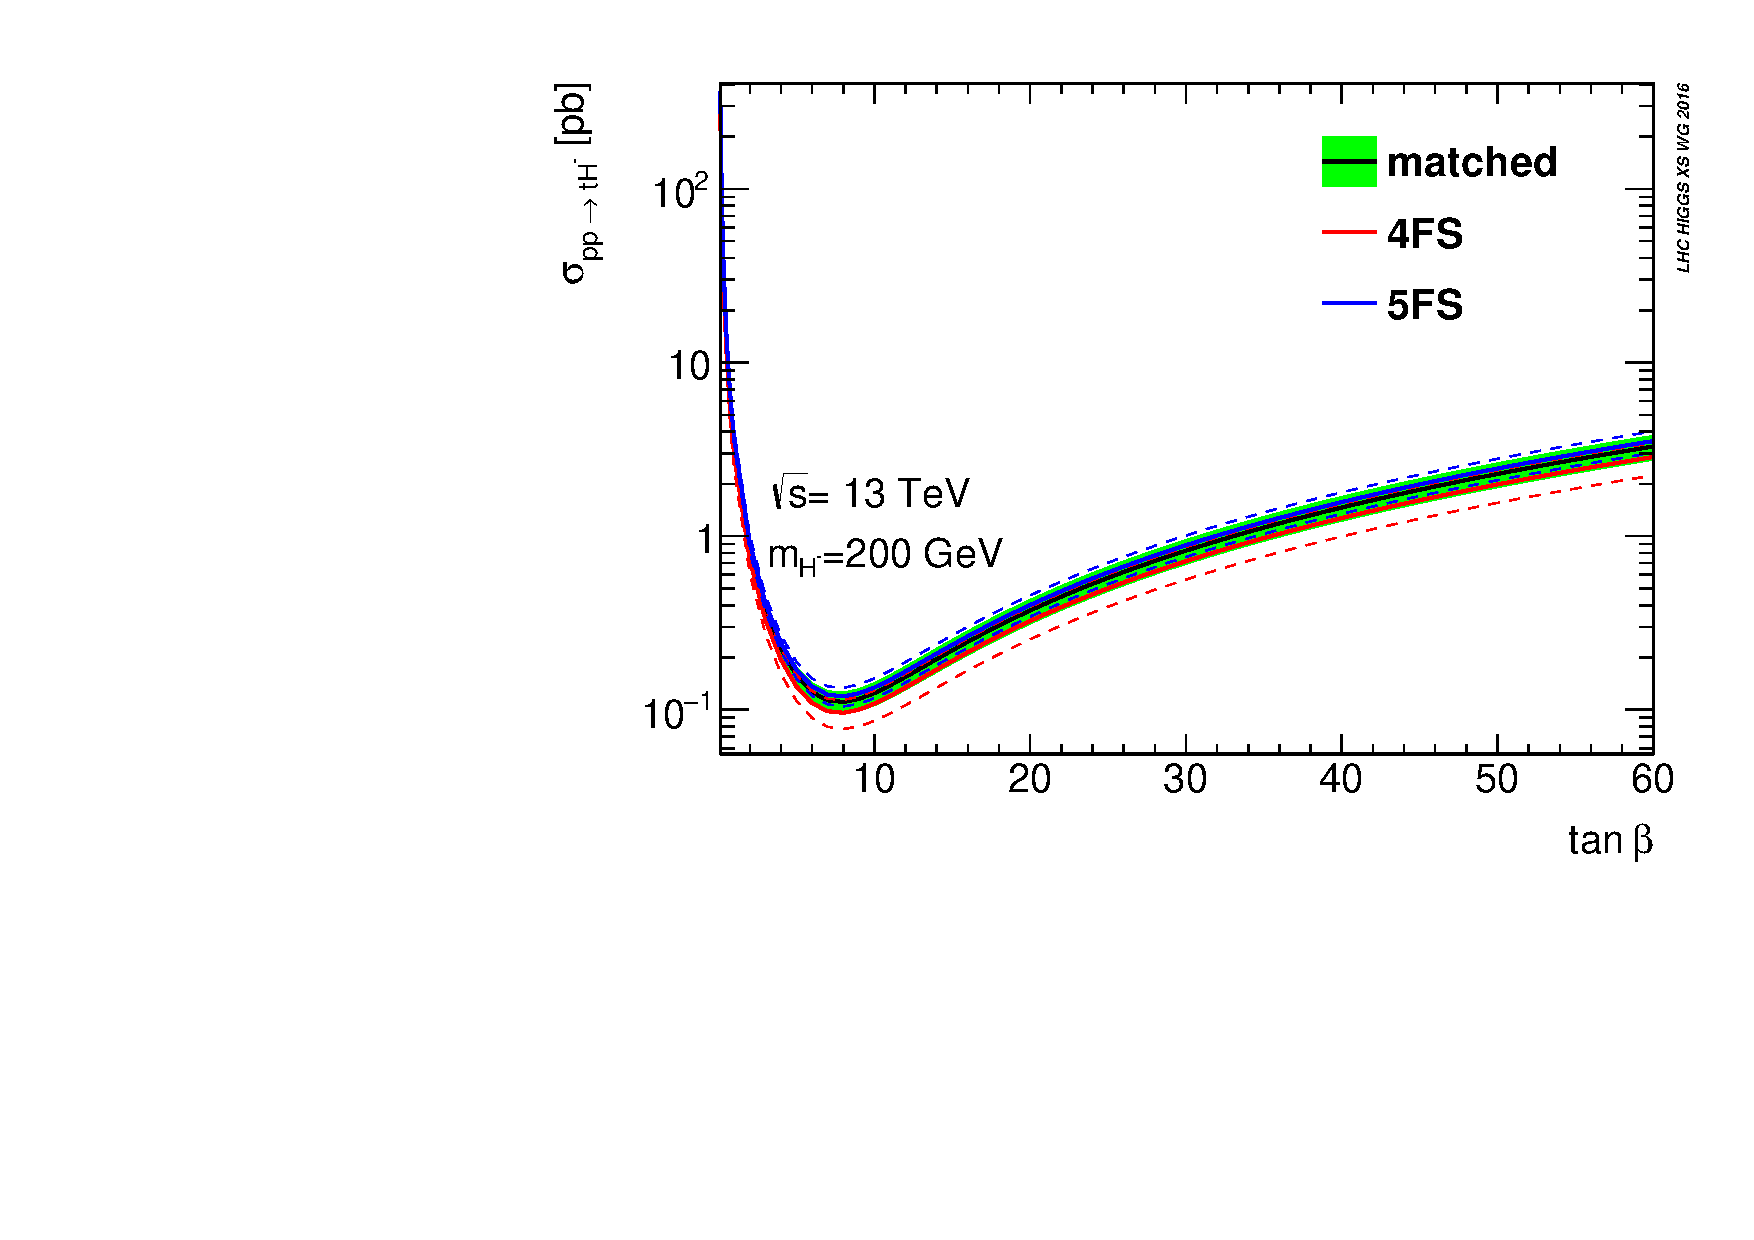
\includegraphics[width=0.5\textwidth]{figures/xsec_mhp_200.pdf}
\caption{Plots of the charged Higgs production cross section against $\tan\beta$ at $\sqs=13~\TeV$ 
collision energy, for $\mcH=200~\GeV$}
\label{fig:chargedHxs}
\end{figure}

\par The \Hplus\ can decay through any of the vertices in Figure~\ref{fig:chargedHverts}. Modes 
with interactions between \Hplus\ and other Higgs bosons in the Higgs sector are very 
low, so they are ignored. Figure~\ref{fig:BR_chargedH} shows branching fractions for the significant 
decay modes for \Hplus\ in the MSSM as a function of \mcH. The $m_h^{\text{mod+}}$ alludes to the fact 
that $h$ is taken with a mass of 125~\GeV, so the branching ratios corresponds to an hMSSM scenario at 
$\tan\beta=10$ and $50$. At both $\tan\beta=10$ and 50 the dominant decay mode is $t\bbar$ for $\mcH>200~\GeV$. 
This is followed by the $\tau\nu_\tau$ mode, which is in fact more dominant at low \mcH. Due to its low 
expected background, with at least 10\% branching ratio the $\tau\nu_\tau$ mode is more attractive 
than the $t\bbar$ mode due to copious background contamination in the latter. The analysis presented 
in this text searches for evidence of \Hplus\ through the $\tau\nu_\tau$ mode. This discussion will 
be revisited in Chapter~\ref{chargedH}. 

\begin{figure}[!h]
\begin{subfigure}{0.5\textwidth}
   \includegraphics[width=\textwidth]{figures/YRHXS3_BR_fig33.eps}
\end{subfigure} % 
\begin{subfigure}{0.5\textwidth}
   \includegraphics[width=\textwidth]{figures/YRHXS3_BR_fig34.eps}
\end{subfigure}
\caption{Charged Higgs decay branching ratios in the hMSSM scenario, where $m_h^{\text{mod+}}$ alludes to 
the fact that $h$ is the observed SM Higgs. Left shows $\tan\beta=10$ and right shows $\tan\beta=50$}
\label{fig:BR_chargedH}
\end{figure}
